\documentclass{bioinfo}
\copyrightyear{2005}
\pubyear{2005}

\begin{document}
\firstpage{1}

\title[short Title]{Seeq: a library for inexact DNA sequence matching}
\author[Zorita \textit{et~al}]{Eduard Zorita\,$^{1,2}$ and Guillaume J. Filion\,$^{1,2}$\footnote{to whom correspondence should be addressed}}
\address{$^{1}$Genome Architecture, Gene Regulation, Stem Cells and
  Cancer Programme, Centre for Genomic Regulation (CRG), Dr. Aiguader
  88, 08003 Barcelona, Spain\\
$^{2}$Universitat Pompeu Fabra (UPF), 08002 Barcelona, Spain}

\history{Received on XXXXX; revised on XXXXX; accepted on XXXXX}

\editor{Associate Editor: XXXXXXX}

\maketitle

\begin{abstract}

\section{Motivation:}
Searching specific sequences in DNA is one of the most common tasks
in the analysis of biological data. Experimental samples often contain
known sequences at the positions where adaptor removal, sequence
trimming or barcode extraction have to be performed. Experimental data
contain errors that must be tolerated in order to identify these
patterns. For reads produced by second generation sequencing,
where the error rates lie below 2\%, short sequences with small error
tolerance suffice to identify the patterns. However, third generation
sequencing technologies promise longer reads at the cost of 10-fold
higher error rates. In this scenario, both the pattern length and the
relative error tolerance have to be dramatically increased.
\section{Results:}
Here we present seeq, an algorithm for pattern matching with errors.
Seeq is optimized for DNA sequences and shows very little variance in
running time with different configurations. We benchmark seeq against
the most widely used algorithms for inexact pattern matching. The
results show that seeq scales better and becomes significantly faster
as the error rate increases.
\section{Availability:}
Seeq is available in three forms: a Linux software, a C library and a 
Python module. The source code and the C/Python libraries are available
for download at
\href{http://github.com/ezorita/seeq}{http://github.com/ezorita/seeq}.
\section{Contact:} \href{guillaume.filion@gmail.com}{guillaume.filion@gmail.com}
\end{abstract}

\section{Introduction}

Inexact string matching dates back to the origin of computer sciences
\citep{Lev65}. The first algorithms addressing this problem were based
on dynamic programming \citep{NW70}. They are still widely used to
align biological sequences due to their simplicity and flexibility.
More sophisticated algorithms derived from the Boyer-Moore search
method \citep{BM77} were later designed to search patterns on long
strings allowing errors. Such algorithms are faster than the dynamic
programming approach because they do not compute all the relative
distances. Instead, the pattern is pre-processed to design a search
strategy which skips parts of the text that do not contain any
match. The jumping strategy is very efficient for perfect matches or
small edit distances because non-matching conditions can be inferred
with only a few comparisons. In such conditions, the number of
operations per input character is small because large areas of the
text are never processed. However, when the error rate is high, the
search strategy requires more comparisons to identify a non-matching
condition. The drop in performance is even more accute when the alphabet
is as small as in the case of DNA sequences.

Illumina reads typically have a 1-2\% error rate,
mainly consisting of substitutions \citep{Doh08}, which are ideal
conditions for the Boyer-Moore algorithm. However, third generation
sequencing technologies such as the PacBio platform now come of age.
They produce reads two orders of magnitude longer than Illumina, at
the expense of a 10-fold higher error rate (15\%) consisting mostly
of insertions and deletions \citep{Eid09}.  
This high error rate dramatically increases the false
positive rate unless the pattern sequence is extended
accordingly. This raises a new scenario with long patterns and
large edit distances.

Here we present \emph{seeq}, an algorithm using a dynamic version of
deterministic finite automata (DFA). Instead of using standard
construction procedures, the dynamic DFA of seeq is built as the input
text is processed. We benchmark seeq against other inexact string
matching software. The results show that seeq scales better and
becomes significantly faster as the error rate increases. 
\begin{methods}
\section{Methods}

We use a DFA representation of a dynamic programming algorithm.
We search the occurrences of the pattern $P$ of length $m$
in a text $T$ of length $n$, with up to $k$ differences.
The edit matrix $\mathbf{C} \in \mathbb{N}^{m\times n}$ is initialized
with $\mathbf{C}(0,j)=0$ and $\mathbf{C}(i,0) = i$, and then updated
column-wise with the Needleman-Wunsch recusrion. Note that this process
can be represented as $\mathbf{c}_j=f(\mathbf{c}_{j-1},T_j)$,
\textit{i.e.} the value of the $j$-th column $\mathbf{c}_{j}$ is a
deterministic transition that only depends on $\mathbf{c}_{j-1}$ and the
character $T_j$. We take advantage of this property to build a
deterministic automaton where the states are the columns of the matrix
and the transitions are dictated by the input characters.
We represent the states of the DFA by the differential encoding
of the $j$-th column, $\mathbf{s}(i)=\mathbf{C}(i+1,j)-\mathbf{C}(i,j)+1$
so that the state can be stored in a ternary trie ($\mathbf{s}(i)$
can take only 3 values).

\begin{figure}[!tpb]
\centerline{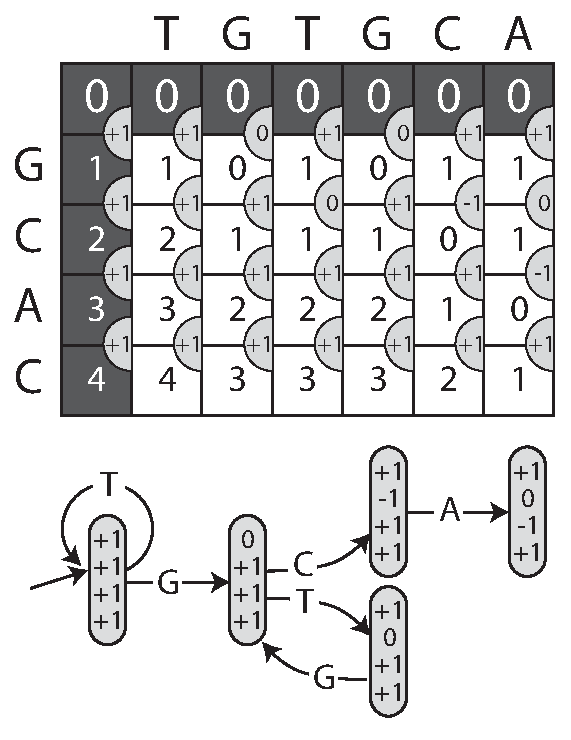
\includegraphics[scale=0.6]{Figure_1.pdf}}
\caption{Dynamic DFA construction process. In this example, the search
text is TGTGCA and the pattern is GCAC.
A) Dynamic programming matrix of the alignment. The differential code
of each column is shown inside the semicircles. B) State of the DFA at
the end of the alignment.}\label{matrix}
\end{figure}

The DFA construction process is illustrated in Figure \ref{matrix}. The
dynamic programming algorithm starts at the DFA state
$S = S_0$. For any input character $T_j$, being $S$
the active DFA state, the algorithm recursively proceeds as follows:
\begin{enumerate}
\item If $S$ has an outgoing path (to $S_q$) with
label $T_j$, then set $S = S_q$.
\item Otherwise, revert $\mathbf{c}$ from $\mathbf{s}$ and compute
the $j$-th column of the edit matrix as $\mathbf{c}_j = f(\mathbf{c}, T_j)$ and
its diferential code $\mathbf{s}_j$. Then: a) If $\mathbf{s}_j$
represents an existing state ($S_q$), connect $S$ to it with a path
labeled $T_j$ and set $S = S_q$. b) If none of the states is
represented by $\mathbf{s}_j$, create $S_j$, connect $S$ to it with a
path labeled $T_j$ and set $S = S_j$.
\end{enumerate}

After several steps, the graph of the DFA is densely connected and
case 2 almost never occurs. The complexity of the algorithm is then
reduced to direct DFA state transitions.

\end{methods}

\section{Results}

We have benchmarked seeq against two standard inexact string
matching algorithms: agrep \citep{Wu92} and nr-grep \citep{Nav01}. We
used two sequencing datasets for benchmarking. Both datasets contain
10 million reads but differ in read length. Dataset 1 consists of random
\textit{Drosophila} genome reads of length 100. The reads of dataset 2
are 50 nucleotides long, from which the first 30 nucleotides are constant
and the last 20 are random (barcodes). The software were set to match
random patterns ranging from 5 to 50 nucleotides with a random error
tolerance up to 40\%. Importantly, agrep limits the number of differences
to 8, which is a serious limitation and makes the comparison fair only
between seeq and nr-grep.

\begin{figure}[!tpb]
\centerline{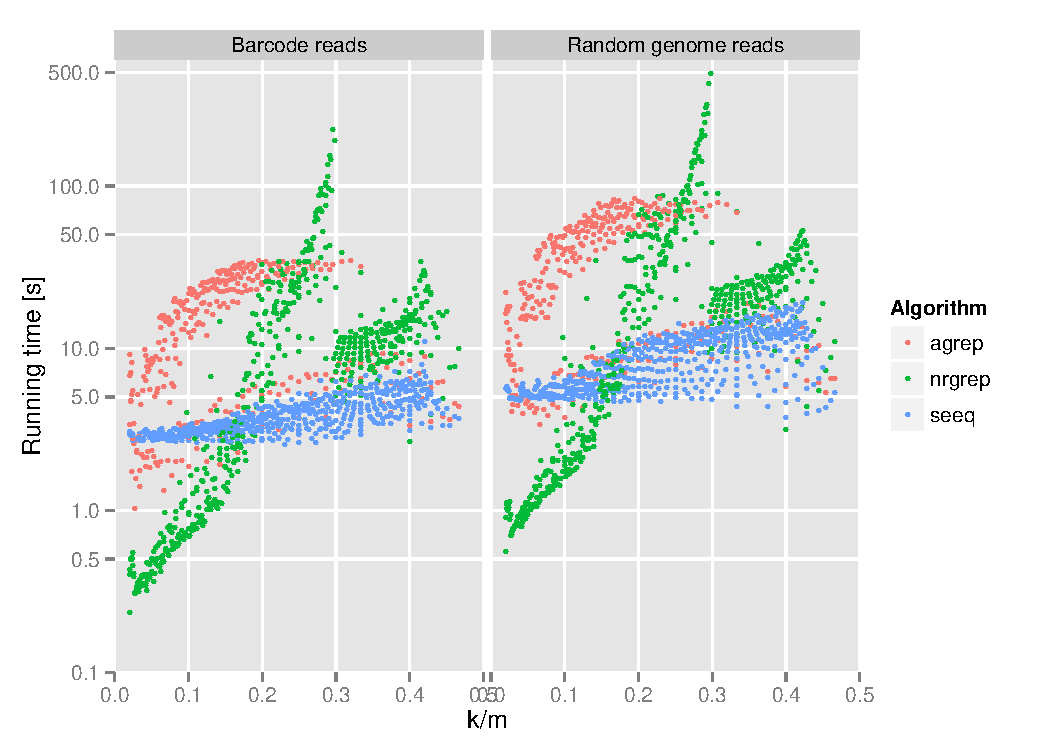
\includegraphics[scale=0.5]{results.pdf}}
\caption{Benchmark between seeq, agrep and nr-grep. Each dot represents
the running time of one search with a random pattern and a random
edit distance. Note the logarithmic scale on the y axis.}
\label{fig:results}
\end{figure}


The running time of each execution is plotted against the relative
error tolerace ($k/m$) on Figure \ref{fig:results}. For low error
rates, both agrep and nr-grep perform better than seeq, with a maximum
5-fold advantage when $k=1$ and $m > 25$. On the other hand, seeq is
up to two orders of magnitude faster than nr-grep and one order of
magnitude faster than agrep for $k/m > 0.15$. The similarity between
the two datasets indicates that neither software is favored when the
data has a repetitive structure. Also note that seeq 
achieves near-constant running time.

\section{Conclusion}

The benchmark shows that seeq is faster in higher error regions with
an excellent worst case. Actually, the running time of seeq depends
very little on the error tolerance. The higher efficiency of seeq
is attributed to the underlying dynamic DFA structure. Here, the key
insight was to take advantage of the limited size of the DNA alphabet.
This strategy is usually not efficient in general string matching
problems.

In practice, most pattern searches in DNA reads are performed from
scripts and pipelines. To ease the use of seeq in existing software,
we have ensured that it is compliant with Linux pipes. Also, we have
created a Python module that can be imported and integrated seamlessly,
as it can be called on Python string objects that can be further
manipulated. We also provide an API in C for the cases that optimal
performance is required.


\paragraph{Funding\textcolon}
The research leading to these results has received funding from the
European Research Council under the European Union's Seventh Framework
Programme (FP7/2007-2013) / ERC SYNERGY n$^\circ$ 609989.


\bibliographystyle{natbib}
%\bibliographystyle{achemnat}
%\bibliographystyle{plainnat}
%\bibliographystyle{abbrv}
%\bibliographystyle{bioinformatics}
%
%\bibliographystyle{plain}
%
\bibliography{document}


\end{document}
